\documentclass{article}

\usepackage{repsty}
\usepackage{wrapfig}

\usepgfplotslibrary{fillbetween}


\begin{document}
	
\section*{Problem statement}

Our goal is to estimate the frequency $\omega$ of the signal
\begin{equation}
	N(t) = N_0\cdot\bkt{1 + P\cdot e^{-\sfrac{t}{\tau_d}}\cdot\sin(\omega\cdot t + \phi)},
\end{equation}
where $\tau_d$ is the spin tune lifetime. One measurement $N_i = N(t_i)$ takes anywhere between 1--10 milliseconds, and involves two to three thousand detector counts (Y. Senichev, personal communication Dec 9, 2016).

Assuming the Normal error distribution with mean zero and variance $\nu = \SD{\meas}^2$, the maximum likelihood estimator for the variance of the frequency estimate can be expressed as
\begin{equation}
\begin{cases}
\var{\hat\omega} &= \nu\bkt{\sum_j x_j\cdot \var[w]{t}}^{-1}, \\
\var[w]{t} &= \sum_i w_i \bkt{t_i - \avg{t}_w}^2,~ \avg{t}_w = \sum_i t_i w_i, \\
w_i &= \frac{x_i}{\sum_j x_j},~ x_i = (N_0P\exp(\lambda t_i))^2\cos^2(\omega t_i + \phi) = \bkt{\mupp}^2.
\end{cases}	
\end{equation}

The three factors, contributing to the standard error of the estimate are:
\begin{inparaenum}[\itshape a\upshape)]
	\item the error variance $\nu \equiv \SD{\meas}^2$ (governed by the number $\Ncm$ of detector counts per measurement), 
	\item the time spread $\sum_i w_i (t_i - \avg{t}_w)^2$ of the sample measurements, and
	\item their net informational content $X_{tot} = \sum_i \bkt{\mupp}^2$.
\end{inparaenum}

The latter two quantities are related as a consequence of spin tune decoherence: in order to increase the measurement time spread, one has to raise the beam lifetime, which in turn increases the proportion of less informative measurements in the sample. The error variance is related to the time spread by virtue of 


The variance is inversely proportional to the (weighted) spread of the predictor variable, and directly proportional to the variance of the error. 

Regarding the former, the weighting by the derivative of the signal has a twofold effect: in the first place, measurements that are taken when the derivative is maximal contribute more to the spread than those made when the signal changes slowly. Considering the number of possible measurements during a fill is limited, a more cost-effective use of the beam is a concern; one that could be addressed by sampling only during the periods of rapid change in the signal. In the second place, due to spin tune decoherence, the measurements' contribution goes down with time. This aspect restricts our ability to maximize sampling efficiency. A possible trade-off would be to reduce the number of counts involved in, and thus the time of, taking a measurement. That way, more measurements could be squeezed in the periods when the sine changes sign (node), but simultaneously, the uncertainty of a measurement would be increased. 

The above considerations prompt the following series of questions:
\begin{enumerate}
	\item How long to measure the signal?
	\item How many counts per measurement are optimal?
	\item How congregated about the signal nodes the measurements should be?
\end{enumerate}
We will try to answer them in what follows.

\section{Spin tune decoherence time}
A rough estimate of the maximum sensible experiment duration could be done by considering the time when the signal oscillation is indistinguishable from noise. If we denote by $\SD{\meas}$ the standard deviation of measurement error, sensibility would require
\[
N_0P\cdot e^{-\sfrac t\tau_d} \geq Z_\alpha \SD{\meas}.
\]
Then 
\[
t_{max} = \tau_d\cdot \log\bkt{Z_\alpha^{-1}\frac{N_0P}{\SD{\meas}}}.
\]

At a three percent error $\SD{\meas} = 3\%\cdot N_0P$ the signal will be indistinguishable from noise at three standard deviations ($Z_\alpha = 3$), by $t_{max} = 2.4\cdot \tau_d$. 

%We have the Cram\'er-Rao inequality to tell us what's the minimum variance of an estimator is possible:
%\[
%	\var{\hat{\omega}} \geq \frac{1}{\Fisher(\omega)}.
%\]
%Fisher information is additive, and what I call \emph{point Fisher information} can be expressed as:
%\[
%	\Fisher[i] = \frac{1}{\nu}\begin{pmatrix}
%		\bkt{\sqrt{2}\cdot\mupp}^{-2} & 0     & 0   \\
%		0                             & t_i^2 & t_i \\
%		0                             & t_i   & 1
%	\end{pmatrix}\cdot \bkt{\mupp}^2.
%\]
%
%\begin{wrapfigure}{l}{.25\textwidth}
%	\begin{tikzpicture}
%	\draw[->] (-1.5,0) -- (1.5,0) node[right] {$\mupp$};
%	\draw[->] (0,-.5) -- (0, 2.3) node[above] {$I_i(\pars_0)$};
%	\draw[scale=1,domain=-1.5:1.5,smooth,variable=\x,red] plot ({\x},{\x*\x});
%	\end{tikzpicture}
%\end{wrapfigure}

\section{Number of counts per measurement}

Define the following variables: \begin{inparaenum}[\itshape a\upshape)]
	\item the number of counts per measurement: $\Ncm$;
	\item the number of measurements per node: $\Nmnd$;
	\item the number of nodes per experiment: $\Nnd$.
\end{inparaenum}

The expected total number of scatterings in an experiment with a given number of nodes: $n_{tot} = \underbrace{\Nnd\cdot\Nmnd}_{\Nm}\cdot\Ncm$. ($\Nm$ is the total number of measurements.)

\begin{equation}
\begin{cases}
	\SE{\hat{\omega}}^2 &= \frac{\SD{\meas}^2}{X_{tot}\cdot\sum_{j=1}^{\Nm}w_j\bkt{t_j - \avg{t}_w}^2}, \\
	\SE{\meas}^2 &= \frac{\SD{\meas}^2}{\Ncm} ,\\
	X_{tot} &= \sum_{j=1}^{\Nm} x_j = \sum_{s=1}^{\Nnd}\sum_{j=1}^{\Nmnd} x_{js}.
\end{cases}
\end{equation}

We can express $\sum_{j=1}^{\Nmnd} x_{js} = \Nmnd \cdot x_{0s}$, for some mean value $x_{0s}$ in the given node $s$. The sum $\sum_{j=1}^{\Nmnd} x_{js}$ falls exponentially due to decoherence, hence $x_{0s} = x_{01}\exp{(\lambda\cdot \frac{(s-1)\cdot\pi}{\omega})}$. Therefore,
\[
	X_{tot} = \Nmnd\cdot x_{01} \cdot \frac{\exp{\bkt{\frac{\lambda\pi}{\omega}\Nnd}}-1}{\exp{\bkt{\frac{\lambda\pi}{\omega}}}-1} \equiv \Nmnd \cdot g(\Nnd).
\]

\begin{figure}[h]
	\centering
	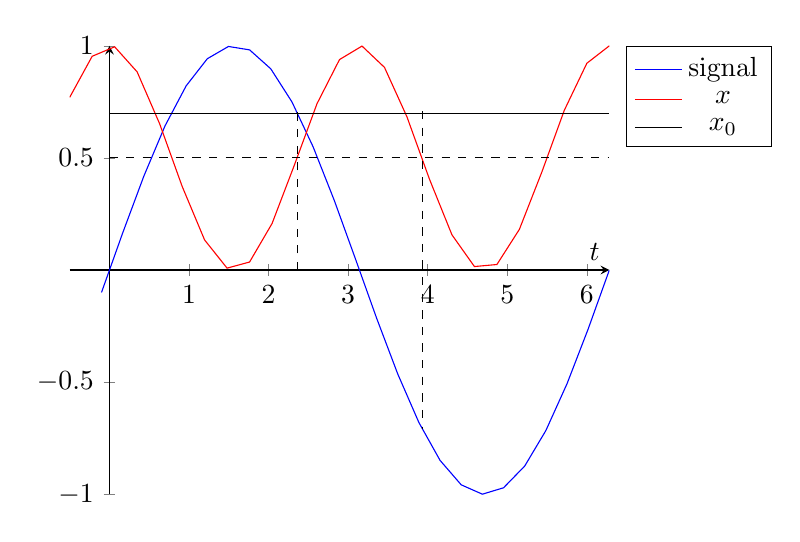
\begin{tikzpicture}
		\begin{axis}[axis lines=center, xlabel=$t$, domain=-.5:2*pi, legend pos=outer north east]
		\addplot[color=blue, name path=signal, domain=-.1:2*pi] {sin(deg(x))}; \addlegendentry{signal}
		\addplot[color=red] {cos(deg(x))^2}; \addlegendentry{$x$}
		\addplot[mark=none, domain=0:2*pi]{.7}; \addlegendentry{$x_0$}
		\addplot[mark=none,dashed, domain=0:2*pi]{.5};
		\draw[dashed] (axis cs:2.36,0) -- (axis cs:2.36,{sin(deg(2.36))});
		\draw[dashed] (axis cs:3.93,{-sin(deg(3.93))}) -- (axis cs:3.93,{sin(deg(3.93))});
		\end{axis}
	\end{tikzpicture}
	\caption{Explanation for $x_0$\label{fig:x0Expl}}
\end{figure}

The number of events per node 
\[
	\Nmnd = \frac{\Delta t_{zc}}{\Ncm\cdot \Delta t_{\cnt}},
\]
hence
\[
	X_{tot} = g(\Nnd) \cdot \frac{\Delta t_{zc}}{\Delta t_{\cnt}}\cdot \frac{1}{\Ncm}.
\]

The variance $\var[w]{t}$ is also practically independent of how many measurements there are per one node (and by extension, the number $\Ncm$), and depends primarily on the $\Nnd$ and decoherence life time.

In sum, assuming one measurement is the mean of the counts ($\SD{\meas} = \SD{\meas}/\sqrt{\Ncm}$), 
\begin{align*}
	\var[w]{\hat{\omega}} &= \frac{\SD{\meas}^2\cdot \sfrac{1}{\Ncm}}{g(\Nnd)\cdot \frac{\Delta t_{zc}}{\Delta t_{\meas}}\cdot \sfrac{1}{\Ncm} \cdot \var[w]{t}} \\
		&= \frac{\SD{\meas}^2}{g(\Nnd)\cdot \frac{\Delta t_{zc}}{\Delta t_{\meas}} \cdot \var[w]{t}}.
\end{align*}
There's no benefit to increasing the number of counts per measurement.

\section{Modulation}
% THE OLD VERSION
% is based on the results of the previous section; the premises that var(measurement) = var(count)/number_of_counts and that the informativity of measurements in one region can be uniformalized to x01 %%%%%%

%In order to increase beam use efficiency, it is advantageous to sample the signal only during rapid change. That way, the yield of Fisher information per scattered particle is maximized. However, one has to take into account that the beam polarization dissipates continuously, whether the beam is being sampled or not, and so there's a finite window in which sampling yields statistically significant results. We will estimate how long that is in the next section, but for now we will assume that it is less than the beam lifetime when it is scattered continuously.
%
%Then frequency-modulated sampling will perform worse than uniform sampling. That is because, unless measurements are made proportionally faster, there will be fewer points sampled by the time the signal is indistinguishable from noise. But an increase in sampling frequency would not have any effect on the result, because measurement variance is increased proportionally.

% THE NEW VERSION begins here
\newcommand{\dt}{\Delta t}
\DeclareDocumentCommand{\stat}{s}{\IfBooleanTF{#1}{\alpha}{\frac{\SD{\meas}^2}{\SE{\hat\omega}^2\cdot \var[w]{t}}}}
\begin{align*}
	X_{tot}	&= \Nmnd\cdot \tilde{g}(\Nnd)\cdot x_{01}, \\
	X_{tot}	&= \stat = \stat*, \\
	x_{01}	&= \int_{-\dt/2}^{+\dt/2}\cos^2(\omega\cdot t)\td t = \frac12\cdot \bkt{\dt + \frac{\sin\omega\dt}{\omega}}.
\end{align*}

\begin{align*}
	\dt + \frac{\sin\omega\dt}{\omega}	&= 2\cdot \stat* \cdot \bkt{\Nmnd\cdot \tilde{g}(\Nnd)}^{-1}, \\
	\Nmnd	&= \frac{\dt}{\dt_{meas}}.
\end{align*}

\end{document}